\documentclass[
	%a4paper, % Use A4 paper size
	letterpaper, % Use US letter paper size
]{jdf}

\addbibresource{references.bib}

\author{Author Name}
\email{username@gatech.edu}
\title{Joyner Document Format v2.2:\\For Use in CS6460, CS6750, and CS7637}

\begin{document}
%\lsstyle

\maketitle

\begin{abstract}
	Welcome to Joyner Document Format (JDF) v2.2! JDF is primarily intended to standardize page lengths while ensuring readability. Note that you are required to use JDF for all written assignments, but we will not perform explicit formatting checks. So, while improper formatting may be subject to penalties, you should not worry too much about whether your submission conforms to every minute detail; the most important elements are margins, font, font sizes, and line spacing. Just make a copy of one of the provided templates and replace its contents with your own, using the built-in paragraph styles.\footnote{Here are instructions for \href{https://support.office.com/en-us/article/Video-Using-Styles-in-Word-9db4c0f4-2754-4294-9758-c14a0abd8cfa}{Microsoft Word}, \href{https://support.apple.com/guide/pages/intro-to-paragraph-styles-tanaa39b0aa3/mac}{Apple Pages}, and \href{https://www.bazroberts.com/2016/04/19/google-docs-paragraph-styles-headings/}{Google Docs}.} If you do so, you do not need to verify that the style was followed.
\end{abstract}

\section{Typography}
All text in JDF should be set in the Palatino typeface. It is available practically everywhere as a system font: Microsoft ships a version called \emph{Palatino Linotype}, and Apple uses a version simply called \emph{Palatino}. Those without either can look for \emph{Book Antiqua} in their fonts list or download \href{https://www.ctan.org/tex-archive/fonts/tex-gyre/opentype}{\TeX\ Gyre Pagella} from CTAN. They all come in regular and bold weights with matching italics.

\subsection{Body text}
Body text is set in the regular weight at 11 points with 17 points of line spacing, and 8.5 points of spacing added after each paragraph. It should be justified with hyphenation enabled where available. Paragraphs should not be indented. These styles can be automatically applied using the \emph{Normal} paragraph style.

\textbf{Bold} and \textit{italics} should be used for emphasis. Hyperlinks may be inserted in the text, as well as {\tt in-line code}, superscripts\textsuperscript{ like this}, and subscripts\textsubscript{ like this}.

\subsection{Title \& subtitle}
The paper title should be set in the regular weight at 17 points with 22 points of line spacing, centered at the top of the first page. The title may span up to three lines. For typical assignments, the document title may be as simple as “Assignment 1” More specialized assignments may warrant more unique paper names, like “A Proposal to Create a New Document Format.”

The author’s name and email should come next unless you want to or were asked to submit anonymously, in which case this can be omitted. They should be set in the same size and weight as body text, centered. These styles can be applied using the \emph{Title} and \emph{Subtitle} paragraph styles.

\subsection{Abstract}
If your paper requires an abstract, it should be placed at the top of the first page underneath the title block, preceded by the word \emph{Abstract} in bold italic. An extra 0.5" should be added to both sides. Not all papers require abstracts; only those that would benefit from a high-level summary of the project or its background.

\subsection{Headings}
Headings should all be set in the same size as body text (11 pt) in bold. With the exception of \emph{Heading 1}, they should all have 8.5 pt of space before and after. They should be hierarchically numbered: Word, Pages, and \LaTeX\ will do this automatically when you use the appropriate paragraph styles, but Google Docs users will need to number their headings manually. Headings should not span more than one line.

\subsubsection{Heading 1}
Heading 1 should be set in all caps, with letterspacing expanded by 0.66 points (6\%). It should have 11 points of space added before and 8.5 points of space added after.

\subsubsection{Headings 2\,–\,4}
Besides \emph{Heading 1}, which is set in caps, headings should always use sentence case (i.e., first word capitalized) rather than title case; after all, they are not titles. \emph{Heading 2} should be set in bold roman (upright), and \emph{Heading 3} should be set in bold italics. The use of headings beyond \emph{Heading 3} is discouraged.

\subsubsubsection{Heading 4}\emph{Heading 4} is provided as a run-in sidehead. Like \emph{Heading 3}, it is set in bold italics, but it should be followed by an em dash and flow right into the text, as seen at the beginning of the current paragraph. It should be used more as a list style than a heading style, e.g. to set off a list of principles in a heuristic evaluation.

\subsection{Page layout}
JDF uses the US Letter paper size (8.5" x 11"). It has a top margin of 1", and bottom and side margins of 1.5". This yields a text block of 5.5" x 8.5", which is exactly \(\frac{1}{2}\) the size of the page, divided lengthwise.

The page number should be included in the bottom margin, 1" from the bottom of the page – this creates symmetry with the top margin. No other elements should be placed in the margins.

\section{Presentational elements}
You are encouraged to use presentational elements liberally, as long as they add to the clarity of your submissions. They often require less space and fewer accompanying words to explain a given concept, and do a far better job of it.

\subsection{Figures}
Figures should always be centered on the page, although they may also take up the entire width and height of the text block. Figures should always be referenced in the text, and they should include a descriptive caption. Figures may also be equations, diagrams, or other kinds of content.

If your figure includes a white background (e.g. an interface design or graph), it may aid legibility to add a \(\frac{1}{4}\)-point black border.

\begin{figure}[h]
	\centering
	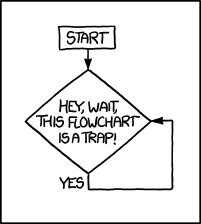
\includegraphics[height=6cm]{Figures/flowchart.png}
	\caption{Make sure your flowcharts are more useful than this one. Source: \href{https://xkcd.com/1195/}{XKCD}.}
	\label{fig:flowchart}
\end{figure}

Figure captions should be centered beneath the corresponding figure. The label (e.g. “Figure 1”) should be set in bold italics followed by an em dash, and the entire caption should be 8.5 pt with 14 pt of line spacing. The \emph{Figure Caption} style in Word will number your figures automatically. If need be, you may have one figure caption corresponding to consecutive figures and use either locational descriptors (e.g. “top left,” “middle”) or labels (e.g. “A”, “B”) to map parts of the caption to parts of the figure. Make sure captions fall on the same page as the corresponding figure or table; you may rearrange text to make this work.

In Word, you may need to either change the image’s text wrap settings to “Top and Bottom” or change the line spacing of the image to 1.0.

\subsection{Tables}
You have freedom to format tables in the way that works best for your data. Generally, text should be left-aligned and numbers should be right-aligned or aligned at the decimal – you can do this using a custom tab stop. The default table style (shown below) reduces the text size to be equal to the caption text.

Table captions should be formatted the same way as figure captions, but they should be placed above the table. The popular mnemonic for this is: figures at the foot, tables at the top. Like figures, tables should not exceed the margins and should be centered on the page.

\begin{table}[h] % [h] forces the table to be output where it is defined in the code (it suppresses floating)
	\caption{Mathematical constants. Notice how the approximations align at the decimal.}
	\small % Reduce font size
	\centering % Centre the table
	\begin{tabular}{L{0.17\linewidth} C{0.12\linewidth} L{0.17\linewidth} L{0.4\linewidth}}
		\textbf{Name} & \textbf{Symbol} & \textbf{Approximation} & \textbf{Description} \\
		\toprule[0.5pt]
		Golden ratio & $\phi$ & 1.618 & Number such that the ratio of " to the number is equal to the ratio of its reciprocal to 1\\
		\midrule
		Euler's number & $e$ & 2.71828 & Exponential growth constant\\
		\midrule
		Archimedes' constant & $\pi$ & 3.14 & The ratio between circumference and diameter of a circle\\
		\midrule
		One hundred & A+ & 100.00 & The grade we hope you’ll all earn in this class\\
	\end{tabular}
\end{table}

\subsection{Additional elements}
There are additional elements you may want to include in your paper, such as in-line or block quotes, lists, and more. For other content types not covered here, you have flexibility in determining how it should be used in this format.

\subsubsection{Quotes}
If you would like to quote an outside source, you may do so with quotation marks followed by a citation. If a quote is fewer than three lines, you may write it in-line. It is acceptable to replace pronouns with their target in brackets for clarity. For example, “Heavy use of peer grading would compromise [the school’s] reputation” (Joyner, 2016). If a quote exceeds three lines, you should set it as its own paragraph with 0.5” side margins, using the Blockquote style.

\begin{quotation}
	\noindent “Whether or not the grades generated by peers are reliably similar to grades generated by experts is only one factor worth considering, however. Student perception is also an important factor. A recent study indicated that reliance on peer grading is one of the top drivers of high MOOC dropout rates. This problem may be addressed by reintroducing some expert grading where possible.” %\citep{joyner2016}
\end{quotation}

\subsubsection{Lists}
Bulleted and numbered lists are indented 0.5" from the left margin, with the bullet or number hanging in the margin by 0.25" (the default format).

Bullet points:

\begin{itemize}
	\item First bullet point item
	\item Second bullet point item
\end{itemize}

Numbered list:

\begin{enumerate}
	\item First numbered item
	\item Second numbered item
\end{enumerate}

\section{Procedural elements}
\subsection{In-line citations}
Articles or sources to which you refer should be cited in-line with the authors’ names and the year of publication.\footnote{In-line citations are preferred over footnotes, and we favor APA citation format for both in-line citations and reference lists. Refer to the Purdue Online Writing Lab, or follow the above examples. Footnotes should use 8.5 point text with 14 point line spacing.} The citation should be placed close in the text to the actual claim, not merely at the end of the paragraph. For example: students in the OMSCS program are older and more likely to be employed than students in the on-campus program \citep{joyner2017}. In the event of multiple authors, list them. For example: research finds sentiment analysis of the text of OMSCS reviews corresponds to student-assigned ratings of the course \citep{newman2018}. You may also cite multiple studies together. For example: several studies have found students in the online version of an undergraduate CS1 class performed equally with students in a traditional version (\cite{joyner2018a}; \cite{joyner2018b}). If you would like to refer to an author in text, you may also do so by including the year (in parentheses) after the author’s name in the text. If a publication has more than 4 authors, you may list the first author followed by ‘et al.’ For example: \citeauthor{joyner2016} (\citeyear{joyner2016}) claim that a round of peer review prior to grading may improve graders’ efficiency and the quality of feedback given. This applies to parenthetical citations as well, e.g. \citep{joyner2016}.

\subsection{Reference lists}
References should be placed at the end of the paper in a dedicated section. Reference lists should be numbered and organized alphabetically by first author’s last name. If multiple papers have the same author(s) and year, you may append a letter to the end of the year to allow differentiated in-line text (e.g. Joyner, 2018a and Joyner, 2018b in the section above). If multiple papers have the same author(s), list them in chronological order starting with the older paper. Only works that are cited in-line should be included in the reference list. The reference list does not count against the length requirements.

\section{References}
\printbibliography[heading=none]

\section{Appendices}
You may optionally move certain information to appendices at the end of your paper, after the reference list. If you have multiple appendices, you should create a section with a \emph{Heading 1} of “Appendices.” Each appendix should begin with a descriptive \emph{Heading 2}; appendices can thus be referenced in the body text using their heading number and description, e.g. “Appendix 5.1: Survey responses.” If you have only one appendix, you can label it with the word “Appendix” followed by a descriptive title, e.g., “Appendix: Survey responses.”

These appendices do not count against the page limit, but they should not contain any information required to answer the question in full. The body text should be sufficient to answer the question, and the appendices should be included only for you to reference or to give additional context. If you decide to move content to an appendix, be sure to summarize the content and note it in relevant place in the body text, e.g., “The raw data can be viewed in \emph{Appendix 5.1: Survey responses}.”

\end{document}